\documentclass[11pt,a4paper]{article}
\usepackage[utf8]{inputenc}
\usepackage[spanish]{babel}
\usepackage{apalike}
\usepackage{amsmath}
\usepackage{amsfonts}
\usepackage{amssymb}
\usepackage{graphicx}
\usepackage[left=2cm,right=2cm,top=2cm,bottom=2cm]{geometry}
\title{Universidad Politécnica de la Zona Metropolitana de Guadalajara}
\begin{document}

\maketitle

\begin{figure}[h]
\begin{center}

\includegraphics[scale=1]{1.jpeg}
\end{center}
\end{figure}

\begin{center}
\author{Sistemas Electrónicos de Interfaz\\
Barrera Vazquez Omar\\
Ing. Mecatrónica 4B}
\end{center}

\newpage

\section{Amplificadores operacionales}

Los amplificadores operacionales son encapsulados que sus principios de funcionamiento se les denomino así por la capacidad de realizar operaciones matemáticas, como suma resta y hasta ecuaciones diferenciales. Actualmente con la entrada de los sistema digitales y los microprocesadores se piensa que esta parte de la electrónica analógica no tiene caso estudiarla, pero sus serias ventajas de en cuanto costos y resistencia de circuito lo hacen un buen elemento en la electrónica de interfaz.

En cuanto los amplificadores y sus tipos de encapsulados vienen en diferentes presentaciones, desde el desarrollo de un solo amplificador para una función en especifica, hasta encapsulados donde pueden venir mas de dos amplificadores para funciones mas avanzadas en la cual pueden compartir fuente de alimentación y conexiones a masa. Ejemplos de lo que se puede utilizar los amplificadores operacionales son los siguientes:

\begin{itemize}
\item Capacidad de alta corriente, alto voltaje o ambos
\item Módulos de envió y recepción para sonar
\item Amplificadores multiplexados 
\item Amplificadores de ganancia programables
\item Automatización y control automotrices
\item Circuitos integrados para comunicaciones
\item Circuitos integrados para radio, audio y video
\item Circuitos integrados para electrometros usados en circuitos con impedancia de entrada muy elevada
\item Circuitos integrados que funcionan con una sola fuente de alimentación
\item Circuitos integrados que funcionan con fuentes de alimentación bipolares
\end{itemize}

En el mundo de los amplificadores operacionales hay distintos tipos para múltiples funciones o funciones en especifico, lo hay de \emph{comparador, sumador, de lazo abierto y lazo cerrado}. En este caso estudiaremos uno de uso común para entender mas su funcionamiento y sus partes que lo componen en un encapsulado, como lo muestra la figura 1:

\begin{figure}[h]
\begin{center}
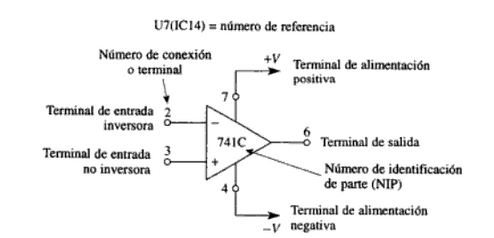
\includegraphics[scale=0.8]{1.png}
\caption{amplificador operacional 741 y sus pines}
\end{center}
\end{figure}

\newpage

Como se observa en el anterior esquema de un amplificador \emph{741} en cual es de uso de excelencia por su bajo costo y alta resistencia, se observan que mantiene cinco pines los cuales tienen una función especifica para el amplificador:

\begin{itemize}

\item \textbf{Terminal de entrada inversora:} en esta parte puede entrar un voltaje que dependiendo el modo que se vaya utilizar el amplificador, puede ser comparado con la entrada no inversora.

\item \textbf{Terminal de entrada no inversora:} al igual que la entrada inversora dependerá mucho de la función que se le este asignando al operador, pero esta también recibe un voltaje.

\item \textbf{Terminal de alimentación positiva:} en esta alimentación puede ser alimentada con un voltaje de 0V o mas voltaje el cual sera una de las opciones a mandar en la salida o amplificar.

\item \textbf{Terminal de alimentación negativa:} al igual que la positiva se convierte en una opción a determinar a la salida del amplificador.

\item \textbf{Terminal de salida:} en esta terminal de salida se obtendrá uno de los dos voltajes que fueron elegidos ya sea positiva o negativa incluso 0V.

\end{itemize}


\section{Modulación de Ancho de Pulso (PWM)}

Un PWM es un tipo de modulación escalar, en cual en un amplificador operacional se obtienen dos señales una señal de referencia y una portadora, en el cual se hace la comparación de las señales y se obtienen dos cosas importantes, \emph{indice de modulación} y \emph{indice de frecuencia, los cuales están dados por las ecuaciones 1 y 2}:

\begin{equation}
m_a=\frac{A_R}{A_C}
\end{equation}

\begin{equation}
m_f=\frac{F_R}{F_C}
\end{equation}

El indice de frecuencia nos dara el tamaño del rizado en la salida y la señal de referencia en diferencia con la conmutacion nos dara diferentes tipos de PWM. Un ejemplo como se observa en la imagen 2:\cite{coughlin1999amplificadores}

\begin{figure}[h]
\begin{center}
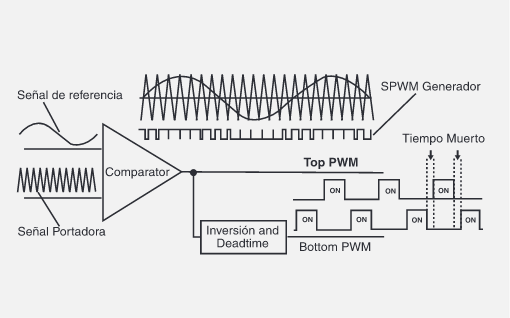
\includegraphics[scale=0.6]{2.png}
\caption{diagrama de escalar PWM}
\end{center}
\end{figure}

\newpage

\section{Diseño de PWM con Amp-Op y transistores}
Un ejemplo de \emph{diseño de modulacion de ancho de pulso} en las codificacion de la entrada de señales ya sea sinusoidal o cuadrada en la cual se ve afectada con una variacion, esto se utiliza normalmente para el area de comunicaciones, donde se tienen diferentes indices de entrada y una seña de referencia en la cual es mandada a un tipo de transistor, notar que se provoca un desfase en la salida de aproximadamente 120 grados, lo podemos observar en la figura 3:\cite{contreras2005modulacion}

\begin{figure}
\begin{center}[h]
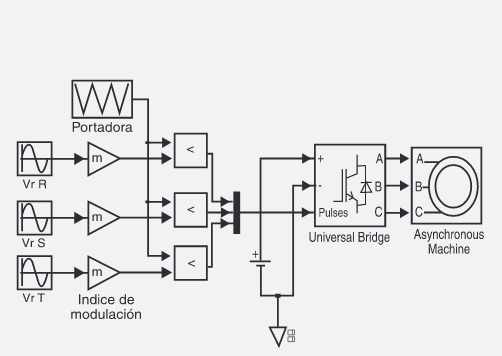
\includegraphics[scale=0.7]{3.png}
\caption{Diagrama en bloques del generador CB-SPWM}
\end{center}
\end{figure}


\bibliographystyle{apalike} 
\bibliography{ref}





\end{document}